% ---------------------------------------------------------------------------
% Author guideline and sample document for EG publication using LaTeX2e input
% D.Fellner, v1.12, Nov 01, 2006

\documentclass[]{egpubl}
\usepackage{eg-it2015}

% --- for  Annual CONFERENCE
% \ConferenceSubmission % uncomment for Conference submission
% \ConferencePaper      % uncomment for (final) Conference Paper
% \STAR                 % uncomment for STAR contribution
% \Tutorial             % uncomment for Tutorial contribution
% \ShortPresentation    % uncomment for (final) Short Conference Presentation
%
% --- for  CGF Journal
% \JournalSubmission    % uncomment for submission to Computer Graphics Forum
% \JournalPaper         % uncomment for final version of Journal Paper
%
% --- for  EG Workshop Proceedings
% \WsSubmission    % uncomment for submission to EG Workshop
 \WsPaper         % uncomment for final version of EG Workshop contribution
%
 \electronicVersion % can be used both for the printed and electronic version

% !! *please* don't change anything above
% !! unless you REALLY know what you are doing
% ------------------------------------------------------------------------

% for including postscript figures
% mind: package option 'draft' will replace PS figure by a filename within a frame
\ifpdf \usepackage[pdftex]{graphicx} \pdfcompresslevel=9
\else \usepackage[dvips]{graphicx} \fi

\PrintedOrElectronic

% prepare for electronic version of your document
\usepackage{t1enc,dfadobe}

\usepackage{egweblnk}
\usepackage{cite}

% For backwards compatibility to old LaTeX type font selection.
% Uncomment if your document adheres to LaTeX2e recommendations.
% \let\rm=\rmfamily    \let\sf=\sffamily    \let\tt=\ttfamily
% \let\it=\itshape     \let\sl=\slshape     \let\sc=\scshape
% \let\bf=\bfseries

% end of prologue

% ---------------------------------------------------------------------
% EG author guidelines plus sample file for EG publication using LaTeX2e input
% D.Fellner, v1.17, Sep 23, 2010


\title[HIJSON: interactive indoor mapping]{HIJSON: cartographic document for web modeling 
of interactive indoor mapping}

\author[F. Spini, M. Sportillo, M. Virgadamo, A. Bottaro, E. Marino \& A. Paoluzzi]
       {F. Spini$^{1}$, M. Sportillo$^{1}$, M. Virgadamo$^{1}$, E. Marino$^{1}$, A. Bottaro $^{2}$, and A. Paoluzzi$^{3}$
%        S. Spencer$^2$\thanks{Chairman Siggraph Publications Board}
        \\
% For Computer Graphics Forum: Please use the abbreviation of your first name.
         $^1$Dipartimento di Ingegneria, Universit\`a Roma Tre, Rome, Italy \\
         $^2$Sogei S.p.A., Ricerca e Sviluppo, Rome, Italy \\
         $^3$Dipartimento di Matematica e Fisica, Universit\`a Roma Tre, Rome, Italy 
%        $^2$ Another Department to illustrate the use in papers from authors
%             with different affiliations
       }

\nonstopmode
% ------------------------------------------------------------------------

% if the Editors-in-Chief have given you the data, you may uncomment
% the following five lines and insert it here
%
% \volume{27}   % the volume in which the issue will be published;
% \issue{1}     % the issue number of the publication
% \pStartPage{1}      % set starting page



\usepackage{balance}

\usepackage{graphicx}
\usepackage{caption}
\usepackage{subcaption}
\usepackage{hyperref}

\usepackage{listings}
\usepackage{xcolor}


\colorlet{punct}{red!60!black}
\definecolor{background}{HTML}{FEFEFE}
\definecolor{delim}{RGB}{20,105,176}
\colorlet{numb}{magenta!60!black}

\lstdefinelanguage{json}{
    basicstyle=\small\ttfamily,
    % numbers=left,
    % numberstyle=\scriptsize,
    % stepnumber=1,
    % numbersep=8pt,
    % showstringspaces=false,
    % breaklines=true,
    % frame=lines,
    backgroundcolor=\color{background},
    literate=
     *{0}{{{\color{numb}0}}}{1}
      {1}{{{\color{numb}1}}}{1}
      {2}{{{\color{numb}2}}}{1}
      {3}{{{\color{numb}3}}}{1}
      {4}{{{\color{numb}4}}}{1}
      {5}{{{\color{numb}5}}}{1}
      {6}{{{\color{numb}6}}}{1}
      {7}{{{\color{numb}7}}}{1}
      {8}{{{\color{numb}8}}}{1}
      {9}{{{\color{numb}9}}}{1}
      {:}{{{\color{punct}{:}}}}{1}
      {,}{{{\color{punct}{,}}}}{1}
      {\{}{{{\color{delim}{\{}}}}{1}
      {\}}{{{\color{delim}{\}}}}}{1}
      {[}{{{\color{delim}{[}}}}{1}
      {]}{{{\color{delim}{]}}}}{1},
}

%----macros begin---------------------------------------------------------------
\usepackage{amssymb}
\usepackage{color}

\def\conv{\mbox{\textrm{conv}\,}}
\def\aff{\mbox{\textrm{aff}\,}}
\def\E{\mathbb{E}}
\def\R{\mathbb{R}}
\def\Z{\mathbb{Z}}
\def\tex{\TeX}
\def\latex{\LaTeX}
\def\v#1{{\bf #1}}
\def\p#1{{\bf #1}}
\def\T#1{{\bf #1}}

\def\vet#1{{\left(\begin{array}{cccccccccccccccccccc}#1\end{array}\right)}}
\def\mat#1{{\left(\begin{array}{cccccccccccccccccccc}#1\end{array}\right)}}

\def\lin{\mbox{\rm lin}\,}
\def\aff{\mbox{\rm aff}\,}
\def\pos{\mbox{\rm pos}\,}
\def\cone{\mbox{\rm cone}\,}
\def\conv{\mbox{\rm conv}\,}
\newcommand{\homog}[0]{\mbox{\rm homog}\,}
\newcommand{\relint}[0]{\mbox{\rm relint}\,}

%----macros end-----------------------------------------------------------------
\begin{document}

 \teaser{
  \includegraphics[width=\linewidth]{images/teaser2}
  \centering
 \label{fig:teaser}
 }

\maketitle

\begin{abstract} This paper introduces HIJSON, a novel indoor cartographic document
format with several enhancements. The document is generated using LAR (Linear Algebraic Representation) allowing for cellular complexes with general topology and shape. 
A software framework FIVE is also presented, that relies on HIJSON
documents and is entirely based on web technologies. With respect to current
cartographic formats, HIJSON suggests four major enhancements: (a) exposes a
hierarchical structure; (b) uses local metric coordinate systems; (c) may
import external geometric models; (d) accepts semantic extensions. The
semantic extensions supported by the HIJSON framework architecture encapsulate
the details about communication protocols, rendering style, and exchanged and
displayed information, allowing the HIJSON format to be extended with any sort
of models of objects, sensors or behaviors. 
\end{abstract}


%-------------------------------------------------------------------------
\section{Introduction\footnote{This work was partially
supported by grant 2014/15 from Sogei S.p.A., the ICT company of the Italian
Ministry of Economy and Finance.}}

For environments with massive presence of sensor-equipped (or ``smart")
objects, which realize the IoT (Internet of Things), the interactive indoor
mapping represents an ideal integrated interface for IoT monitoring systems.
To be specific, it can be the container of indoor navigation systems, giving
the user, to be routed across an indoor environment, the opportunity to
interact with objects along the suggested paths. Furthermore, in conjunction
with the advancements in the field of user indoor location, whose efforts are
nowadays focused to realize an integration of positioning systems like GNSS
(Global Navigation Satellite system), Wi-Fi, Bluetooth and LTE (Long Term
Evolution), to support continuos outdoor/indoor navigation by means of
integration of technologies, it represents the most natural interface to
perform realtime access monitoring and multi-person tracking.Web based
tecnologies supporting self and context aweare objects in conjunction  with
location systems represent the enabling piece for the scenario depicted in
figure~\ref{fig:web-of-thing} we are relentlssly moving torward: the Web of
Things.

\begin{figure}[htbp]
\centering
\includegraphics[width=.5\linewidth]{images/webOfThings.pdf}
\caption{Web of Things (2010--2020?).  Image from~\cite{webOfThings:2015}.}
\label{fig:web-of-thing}
\end{figure}


An interactive mapping platform allows the representation of the indoor
environment of  both public or commercial places of vast dimensions, as for
example airports, train stations, shopping malls, and also private buildings
subject to strict access protocols, like warehouses, logistic centers, data
centers, etc. Despite of the growing attention regarding indoor cartography,
efforts to specify open formats for indoor representation are few and partial,
and certainly not intended to support the interactive indoor mapping, which is
conversely the main purpose of this paper.

Research on the cartographic representation of indoor environments is
extensive and heterogeneous with respect to the strategies
applied~\cite{6418876}. Different information sources are used, and accuracy
of the produced solution depends on the adopted approach. In some cases the
information is obtained with automatic or semi-automatic processing of files
that describe the architectural structure of a building, such as BIM (Building
Information Modeling)~\cite{Eastman:2008:BHG:1796500} and/or IFC (Industry
Foundation Classes) that describe a building project [4].  The actual ``de-facto" 
standard in terms of geospatial data representation is the GeoJSON
format, which can be easily used for any type of geographical annotation. In
some cases it has been slightly adapted to be used in indoor environments: it
is the case of the IndoorJSON format.



%-------------------------------------------------------------------------
\subsection{Our contribution}

The focus of this work is the definition of a novel format of cartographic
documents along with the software ecosystem rooted on it. HIJSON (Hierarchical
Indoor JSON) is the name chosen for the new document format; with the
accompanying software framework, aims to realize a mapping between the real
indoor spaces and a virtual interactive web environment. A simple but
effective algorithm to find indoor valid routes is also provided.


% \begin{figure*}[tbh]
%  \centering
%  ~
%  \begin{subfigure}[b]{0.15\linewidth}
%  \includegraphics[width=\textwidth]{images/sogei-a} 
%  \end{subfigure}
% \hfill
%  \begin{subfigure}[b]{0.21\linewidth}
%  \includegraphics[width=\textwidth]{images/building} 
%  \end{subfigure}
% \hfill
%  \begin{subfigure}[b]{0.15\linewidth}
%  \includegraphics[width=\textwidth]{images/sogei-b}
%  \end{subfigure}
%  \caption{office building: 
%  (a) the schematic plan---made of SVG primitives: lines, rects, polygons---possibly obtained via a client UI loading engineering design in background;
%  (b) the automatically generated LAR cellular complex, transformed server-side into HIJSON; 
%  (c)~the mock-up for the automatically generated 3D HIJSON.
%  }
%  \label{fig:sogei}
% \end{figure*}

\subsubsection{Hierarchical structure}

The HIJSON format allows for hierarchical description of indoor spaces,
reflecting a container-contained relationship. This directly implies a neater
representation then the plain linear structure adopted by GeoJSON, being a
perfect analogy of objects contained (i.e. placed) into spaces. Therefore, an
organized arrangement of spaces is allowed by HIJSON, via logical (or even
physical) grouping: concepts like building wings, sections, storeys,
departments, etc. can be directly introduced, in order to reflect into the
document structure the actual logical or physical divisions, categories or
relationships among the modelled spaces. Furthermore, the container-contained
relation enables a recurring use of local reference frames.

\subsubsection{Metric local coordinate system}

Supported by the hierarchical underlying structure, the HIJSON document format
allows the use of local coordinate systems. Hence the shape of all elements
can be conveniently modelled using local coordinates, and then placed in the
right position with respect to the position of the parent (or container)
element applying a rotation, followed by a translation transformation. Another
substantial advantage is represented by the adoption of a metric reference
frame, consequently simplifying the compilation of the document, either
manually generated or produced by software tools. Just remember that the
GeoJSON coordinates are geographical, a pairs of (absolute) latitude and
longitude angles, like the ones provided by GNSS systems. This kind of
coordinates are certainly not particularly user friendly, when positioning a
smart device or a furniture element within a specific building room.

\subsubsection{Hyperlinked geometric models}

\begin{figure}[h]
 \centering
 \includegraphics[width=\linewidth]{images/sogei2} 
 \caption{Office building: 
 (a) the schematic plan ---made of SVG primitives: 
 lines, rects, polygons--- possibly obtained via a client UI 
 loading engineering design in background;
 (b) the automatically generated LAR cellular complex, transformed 
 server-side into HIJSON; 
 (c and d) the mock-up for the automatically generated 3D HIJSON.
 }
 \label{fig:sogei}
\end{figure}

The HIJSON document may further import external geometric models | either of
the buildings themselves or the interior furniture or devices | that are
topologically complete (in the sense of solid modeling [15]) and very compact.
Such models, coming from a source outside the document, are acquired by
hyperlinking JSON files that contain a Linear Algebraic Representation (LAR)
of topology and geometry, to be expanded for visualization or interaction at
any useful level of detail (see figure~\ref{fig:sogei}). The LAR
scheme~\cite{Dicarlo:2014:TNL:2543138.2543294} is characterised by a very
large domain, including architecture, building and
construction~\cite{paoluzziMS:2014}, 2D and 3D engineering meshes, non-
manifold geometric and solid models and meshes, and high-resolution 3D
images~\cite{cadanda:2015}.  The expansion of a LAR model, to be considered as
a general-purpose graphic primitive, may be executed on either the server or
the supervisor client of the HIJSON Web Toolkit architecture (see Section
6.2.1), or even on the Explorer client.


\subsubsection{Semantic extensions} Semantic extensions make the HIJSON format
extendible and customizable, that is able to adequately respond to any need of
objects representation. To define a semantic extension means to allow the
HIJSON document to model an object previously not covered, or even to modify
the behavior of a comprised one. Semantic extensions are to be defined both as
HIJSON format syntax and as HIJSON Toolkit source code. In particular it is
necessary to define respectively a new HIJSON Element and a new HIJSON Class.


%-------------------------------------------------------------------------
\section{Indoor Modeling of Buildings}

The geometric modeling of interior spaces of complex buildings and architectural environments, with the aim of producing a textual document, aimed to be processed by common web mapping tools,  is not a straightforward task. Actually it requires a sequence of modeling steps that demand for different topological and geometrical concepts, introduced and briefly discussed in this section.

%- - - - - - - - - - - - - - - - - - - - - - - - - - - - - - - - - - - - - 
\subsection{Background}

\subsubsection*{Architectural modeling} 
The \emph{architecture} of a \emph{building} is characterized by two interacting and mutually dependent \emph{systems}, respectively relative to (a) the interior/exterior spaces where the humans live and perform their activities and to (b) the manufacts that realize the physical covering of interior spaces and provide the boundaries of exterior spaces. In short, when modeling an urban area including a set of buildings and their indoor spaces, we must consider both the system of \emph{building spaces} and the system of \emph{building components}.

The system of building spaces may be characterized as a partially ordered family $B$ (Building Units) of subsets of elementary spaces $S$ (Space Units). The set $S$ of space units provide a \emph{partition} of the \emph{Building Space}. The set $B$ of building units is a covering, partially ordered by containment, of the Building space providing a hierarchical structure to it.

The system of building components, also called \emph{building fabric}, can be partitioned into the  \emph{building envelope} and the \emph{building partitions}.

The \emph{building envelope} is the physical separator between the conditioned and unconditioned environment of a building, including the resistance to air, water, heat, light, and noise transfer, along to give buildings form, and to provide shelter and security.

The \emph{building partitions}, either horizontal or vertical, enclose the indoor spaces, and are contained within the building envelope. The former are roofs, floors and ceilings; the latter aim to support the horizontal partitions, either massively or by means of a building frame, where the loads are transferred.

\subsubsection*{Cellular complexes and sparse matrices} 

Therefore, to model the indoor space we need to partition the building into \emph{cells} corresponding to the unit spaces, aggregate them to assembly the hierarchical  building units into \emph{cell complexes}, take control of the adjacency relations though suitable \emph{topological operators}, extract the \emph{boundary chains} of either 2D or 3D \emph{chains} of cells, in order to generate the various families of building components, and extract the \emph{coboundary chains} of subsets of 1D cells or 2D cells, to compute the graph of all paths within the building.

A \emph{cell complex} $X$ is a partition of a compact space $S \subset \E^n$ into compact subsets of points, called \emph{cells}, such that the intersection of every pair of cells is either empty or is a \emph{boundary face} of both. The cells have a \emph{dimension}. 0-cells are topologically equivalent (homeomorphic) to single points (vertices), 1-cells to curves (edges), 2-cells to surfaces (faces) and 3-cells to solids.  The set of $d$-cells is denoted as $X_d$, so that $X$ can be seen as a \emph{stratification} $(X_0, X_1, \ldots, X_d)$. With abuse of language we call $X_h$ the $h$-skeleton of $X$, and $K_h: \{1,2,\ldots,n_h\} \to X_h$ the \emph{indexing maps} of $h$-cells $(0\leq h\leq d)$, where $n_h=|X_h|$. 


\begin{figure*}[htbp] %  figure placement: here, top, bottom, or page
   \centering
   \includegraphics[height=0.16\textwidth,width=0.16\textwidth]{images/zigzag1} 
   \includegraphics[height=0.16\textwidth,width=0.16\textwidth]{images/zigzag2} 
   \includegraphics[height=0.16\textwidth,width=0.16\textwidth]{images/zigzag3} 
   \includegraphics[height=0.16\textwidth,width=0.16\textwidth]{images/randomdelaunay1} 
   \includegraphics[height=0.16\textwidth,width=0.16\textwidth]{images/randomdelaunay2} 
   \includegraphics[height=0.16\textwidth,width=0.16\textwidth]{images/randomdelaunay3} 
   \caption{LAR examples: (a) 2-chain of quad cells; (b) boundary 1-chain; (c) oriented boundary; (d) random 2-complex; (e) oriented 1-skeleton; (f) oriented boundary (red).}
   \label{fig:meshes}
\end{figure*}


When the $X_0$ skeleton is embedded into the Euclidean space $\E^d$, providing a one-to-one mapping $\texttt{V}: K_0 \to \E^d$ of 0-cells with the \emph{vertices} array, a piecewice linear shape may be associated to a $h$-cell $\lambda$ via its characteristic function  as a subset of \texttt{V}. Let us remember that given a subset $A$ of a larger set, the characteristic function $\chi(A)$ is defined to be identically one on $A$, and zero elsewhere. 

The cellular complex $X$ can be represented combinatorially  by $d+1$ families of characteristic functions of $h$-cells as subsets of vertices. For the sake of readability, let us use the symbols  \texttt{V}, \texttt{E}, \texttt{F}, \texttt{C} for $K_0$, $K_1$, $K_2$, and $K_3$, respectively, and \texttt{EV}, \texttt{FV}, \texttt{CV} for the binary matrices to be read as ``edges by vertices'', ``faces by vertices'', and ``cells by vertices'', having as rows the images of characteristic functions of 1-, 2- and 3- cells as discrete sets of vertices.

It is well known that subsets of $h$-cells in a cellular complex can be seen as elements of a linear space $C_h$ of \emph{$h$-chains} over the finite field $Z_2 = \{0,1\}$. When the indexing of cells (i.e.~their ordering) is fixed, the \emph{characteristic matrices} \texttt{EV}, \texttt{FV}, \texttt{CV}, that can be seen as maps from cells to vertices, provide the bases for $C_1$, $C_2$, and $C_3$, respectively. 

The boundary operators $\partial_3: C_3 \to C_2$ and $\partial_2: C_2 \to C_1$, computable by transposition, multiplication and filtering of values of two characteristic matrices~\cite{Dicarlo:2014:TNL:2543138.2543294}, provide the basic tool to study the topology of a cellular complex. The product of the $\partial_d$ matrix  times the characteristic vector of a $d$-chain returns the \emph{boundary $(d-1)$-chain} of facets exposed on the border of such subset of $d$-cells.   

Of course, characteristic and boundary matrices are \emph{very sparse}, with sparsity growing fast with the number of cells, since the number of vertices for cells is small and bounded. Therefore, a list of lists of integers suffices to represent such matrices, and special storage methods~\cite{gemmexp}, and in particular the \texttt{CSR} (compressed sparse row)  and \texttt{CSC} (compressed sparse column), will provide fast computation of the boundary facets of \emph{every subset of cells}.



\subsubsection*{LAR: Linear Algebraic Representation} 

A \emph{representation scheme} is a mapping between the mathematical spaces to be represented by a computer system and their symbolic representation in computer memory. 
The \emph{Linear Algebraic Representation} (LAR) scheme~\cite{Dicarlo:2014:TNL:2543138.2543294}, was recently introduced for topological methods to represent and process mesh connectivity information for dimension-independent cellular complexes, including simplicial, cubical, polytopal, and more general (non-convex and non symply-connected) cells. 

The Linear Algebraic Representation (LAR) scheme uses Combinatorial Cellular Complexes (CCC) as mathematical domain~\cite{Basak:2010} and various compressed representations of sparse matrices~\cite{Williams:2007:OSM:1362622.1362674,gemmexp} as codomain.
This scheme works even with the complicated domain partitions---with non-convex and/or non-manifold cells, and cells non homeomorphic to balls---that may arise in Building Information Modeling (BIM) and Geographic Information Systems (GIS) applications. 

Simplicial and cuboidal cell complexes provide the standard mesh representation used in most science and engineering simulations, whereas complexes of possibly non-convex or non-contractible cells may be needed to represent the built environment in software applications for the Architecture, Engineering, and Construction (AEC) sector.


 \begin{figure}[!h]
  \centering
  \begin{subfigure}[b]{\linewidth}
  \includegraphics[width=\textwidth]{images/minimum-data}
  \end{subfigure}
 \\
  \begin{subfigure}[b]{0.48\linewidth}
  \includegraphics[width=\textwidth]{images/minimum-colors-a}
  \caption{}
  \vspace*{4mm}
  \end{subfigure}
  ~
  \begin{subfigure}[b]{0.48\linewidth}
  \includegraphics[width=\textwidth]{images/minimum-colors-b}
  \caption{}
  \vspace*{4mm}
  \end{subfigure}
 \\
  \begin{subfigure}[b]{0.74\linewidth}
  \centering
  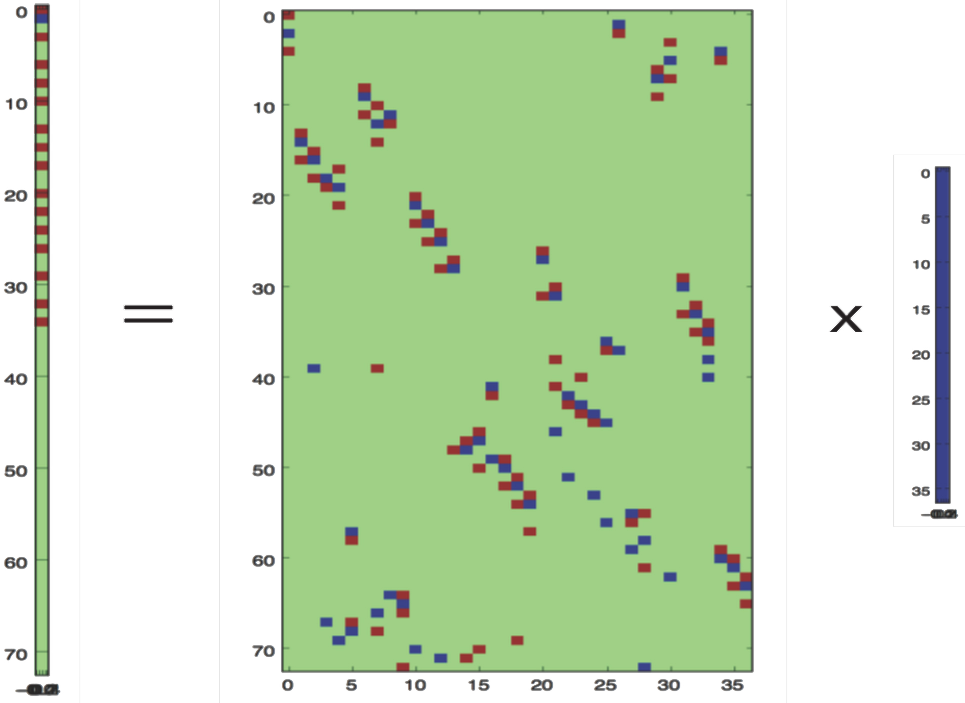
\includegraphics[width=\textwidth]{images/boundary}
  \caption{}
  \end{subfigure}
 
  \caption{A toy example of the LAR scheme: (a) the bare minimum of data with \emph{complete} information about topology; (b) the extracted boundary; (c) the extraction method $[e] = [\partial][f]$ giving the coordinate representation (in the discrete basis of the 1-cells) ofthe boundary edges $[e]$ by product of the sparse boundary operator matrix $[\partial]$ times the coordinate representation $[f]$ of the 2-cells (faces), in the discrete basis of the 2-cells.}
  \label{fig:minimum-data}
 \end{figure}


\subsubsection*{LAR implementation} 

The architectural modeling disussed in this paper is written in Python, using the \texttt{Pyplasm} and \texttt{Lar-cc} libraries.
The application produces \texttt{HIJSON} documents containing 2D plan models of building embedded in 3D (see Figure~\ref{fig:input-png0}b). Those are mapped to complete  3D virtual models, visitable in first person from the client-side  FIVE framework~\cite{Sportillo:2015,Virgadamo:2015}.
The \href{https://github.com/plasm-language/pyplasm}{\texttt{Pyplasm}}  library is a python interface towards a C$^{++}$ geometric kernel, current implementation of the  PLaSM language~\cite{Paoluzzi:1995:GPP:212332.212349,Paoluzzi2003a}, developed as geometric extension of the functional language FL, by Bakus and the functional programming of IBM Research at Almaden~\cite{Aiken91thefl,fl-1,backus:78}. 

The prototype Python implementation \href{https://github.com/cvdlab/lar-cc}{\texttt{lar-cc}} is  in progress as an integral part of a permanent effort to rethink the foundations of solid modeling, by simplifying and generalizing its data representation and disentangling its main algorithms. The computational framework aims to accommodate the new world of geometric data over cloud- and web-based infrastructures. This long-term project has already achieved some tangible results in applications for the extraction of solid models from 3D medical images~\cite{paodcvjcadanda:2015} and to the simplified generation of building models for indoor mapping and IoT (as documented in this paper). 


%- - - - - - - - - - - - - - - - - - - - - - - - - - - - - - - - - - - - - 
\subsection{Hierarchical cellular complex}

aaa aaa aa

\subsubsection*{Boundary and coboundary operators}

\subsubsection*{Building structures and assemblies}

Hierarchical models of complex assemblies are generated by aggregation
of subassemblies, each one defined in a local coordinate system, and
relocated by affine transformations of coordinates.  This operation
may be repeated hierarchically, with some subassemblies defined by
aggregation of simpler parts, and so on, until one obtains a set of
elementary components, which cannot be further decomposed.

Two main advantages can be found in a hierarchical modeling approach. Each elementary part and each assembly, at every hierarchical level, are defined independently from each other, using a local coordinate frame, suitably chosen to make its definition easier. Furthermore, only one copy of each component may be stored in the memory, and instanced in different locations and orientations how many times it is needed.


%- - - - - - - - - - - - - - - - - - - - - - - - - - - - - - - - - - - - - 
\subsection{Production of HIJSON document}

Our RAD of building models is 
obtained via a combination of server-side and client-side computing
based on text-based geometric computing and interactive data 
transformation via graphical input actions. We therefore distinguish
between:

\begin{enumerate}
\def\labelenumi{(\alph{enumi})}
\item
  input of wire-frame drawings from architectural floorplan images into
  standard web representation of vector drawings, followed by parsing of textual (\texttt{.svg}) files;
\item
  generation of a 2D cellular complex for long-term storage
  (\texttt{.lar}) and hierarchical modeling of cellular models using a very simple and general geometric format (LAR) based on algebraic topology methods;
\item
  transformation of the \texttt{.lar} format into a structured 2D
  description providing semantics to spaces and possibly to the
  different elements of the building fabric, by using an object-oriented
  hierarchical interactive description hinged about the concept of
  \texttt{Struct} instance, to be not confused with the structural
  backbone of the building. 
\item
Such structured and semantically annotated
  building model is finally
  exported as a rich textual 2.5-dimensional description using the
  \texttt{HIJSON} format. 
\item
  The \texttt{.json} files are finally transformed client-side into both
  2D and 3D environments allowing the real-time spatial placement and
  user-tracing within the virtual environment of the individuals moving
  inside the real building.
\end{enumerate}

\subsubsection*{From raster images to vector drawings}

The architectural shape is introduced in the system using a rasterization of its plan drawings.
In the test-case we used a \texttt{.png} raster file of the first building floor, and supposed the layout constant on the various storeys. Of course, the number of input files will correspond to the number of different floor plans. In Figure~\ref{fig:input-png} and image is shown of the input image.

An user-interpretation of plans as wire-frame drawings is performed, using some interactive drawing application, producing one or more \texttt{.svg} files, can be written and read by most
interactive drawing applications, both commercial and open-source. Such
files can be also searched, indexed, scripted, compressed, and scripted  using JavaScript. The mechanism of \emph{layers}, if available, is useful to have the building plans correspond exactly. A metric scale is not fixed in advance, since the geometric representation of the building will be subsequently transformed to any useful scale and position by using an affine transformation matrix.

In order to guarantee a standard quality of \emph{datum} for any generated
virtual environment, while at the same time to provide the maximum web 
dissemination of the input process, only a small subset of
\texttt{SVG} primitives is recognized. The
parsing process will understand the \emph{rect}, \emph{line}, \emph{path}, \emph{polygon} and \emph{polyline} elements, as well as any of
their hierarchical aggregation into the container element
\texttt{\textless{}g\textgreater{}}. Transformations applied to the
\texttt{\textless{}g\textgreater{}} element are performed on all of its
child elements. Attributes applied are inherited by child elements. In
addition, it can be used to define complex objects that can later be
referenced by name.

%\begin{figure}[htbp] %  figure placement: here, top, bottom, or page
%   \centering
%   \includegraphics[width=\linewidth]{images/input-png} 
%   \caption{La griglia utilizzata nel disegno ha passo pari a 1 metro lineare.}
%   \label{fig:input-png}
%\end{figure}



\subsubsection*{From vector drawings to cellular complex}

\paragraph*{Line intersection}\label{intersection-of-lines-and-graph-generation}
The first stage concerns the computation of the
intersection points among a set of line segment in the 2D plane. The
containment boxes of the line segments are iteratively classified into nd-tree-like buckets and compared against the 0-dimensional centroid of smaller and smaller buckets of
data.
At the end of the classification, with same geometric object possibly
inserted in several different buckets, a \emph{brute-force} pairwise intersection
is applied to each final subset. Finally, duplicated intersection
points are removed by sorting, and a 1-dimensional LAR data structure is generated,
with 1-cells given by the split line segments.

\paragraph*{Maximal biconnected
subgraph}\label{computation-of-the-maximal-biconnected-subgraph}
It is worth noting that a one-dimensional LAR model is a pair \texttt{(V,EV)} made by an array \texttt{V} of vertex coordinates and by an array \texttt{EV} of pairs of vertex indices, i.e., it is a standard graph representation. the maximal biconnected subgraph is then computed, in order to remove all dangling edges and paths and to generate a plane partition into a set of quasi-disjoint 2D regions. A standard implementation of the Hopcroft-Tarjan algorithm for biconnected graph components~\cite{Hopcroft:1973:AEA:362248.362272} is used for this purpose.


\begin{figure}[htbp] %  figure placement: here, top, bottom, or page
   \centering
   \includegraphics[width=0.469\linewidth]{images/input-png7} 
   \includegraphics[width=0.511\linewidth]{images/input-png12} 
   \includegraphics[width=\linewidth]{images/input-png5} 
   \caption{Immagini leggermente esplose dello 1-scheletro delle strutture gerarchiche a livello di (a) piano-tipo e (b) di aggregato 2.5D di sei piani-tipo.}
   \label{fig:input-png0}
\end{figure}

\paragraph*{LAR of cellular
complex}\label{reconstruction-of-lar-of-the-cellular-complex}

A complete LAR of the plane partition generated by the arrangment of
lines is then computed by traversing in
counter-clockwise order the generated subgraphs, to report the
2-dimensional cells of the plane partition.
In particular, let us consider the binary characteristic matrix \texttt{EV} as the storage for the incidence angles described below, and remark that we represent the edges on the
rows, and the vertices on the columns of the matrix, so that \texttt{EV[h]$=$[K$_1$,K$_2$]} implies $e_h = (v_{k_1},v_{k_2})$ 
and \texttt{EV[h,k$_1$]} is the value stored in 
\texttt{COO$(h,k_i,\alpha)$} when representing the sparse matrix \texttt{EV} in \emph{coordinate format}. 
Hence, we can readily reconstruct the topology of 2-cells by
associating to each non-zero (sparse matrix) element
the angle in radians that the edge $e_h$ forms
with the orizontal line, when this one incides on the vertex $v_k$.
Of course, if $e_h = (v_{k_1},v_{k_2})$, then it will be 
\[
\texttt{EV}(h,k_2) = \texttt{EV}(h,k_1)+\pi = -\texttt{EV}(h,k_1)
\]
This signed angle information is used to traverse the \texttt{EV} graph counterclockwise, and to extract the coherently oriented cycles one by one,
including the exterior cycle. This traversal provides the needed basis for 2-cells, i.e.~the \texttt{FV} matrix. The knowledge of both \texttt{EV} and \texttt{FV} allows to compute the $\partial_2$ matrix, and hence to get a complete control of the floorplan topology.

\subsubsection*{Partial ordering of hierarchical chains}

\paragraph*{Hierarchy of chains}

The next computational stage assign a semantics to 2-cells and to some significant subsets of 1-cells. For this purpose we employ the concept of \emph{hierarchy}.
In mathematics, a hierarchy is a set-theoretical concept, defined as a \emph{preorder} defined on a set. A hierarchy is often defined as either a partially or totally ordered set. All partial orders and equivalence relations are preorders, but preorders are more general. 
In computer science, the term usually refers to \emph{partially ordered sets}, whose elements are classes of objects of growing complexity. In this case the preorder that defines the hierarchy is the \emph{relation of containment} between classes of objects. In this sense we speak of  di \emph{hierarchical chains} as a family of subsets of cells partially ordered by containment.

\paragraph*{Semantics of chains}

The hierarchy of building units, follows from the functional meaning of these, is illustrated by colors in Figure~\ref{fig:input-png6}. We may distinguish in the model floorplan of our model building five 2-chains, orderly corresponding to \emph{north wing}, \emph{south wing}, \emph{east wing}, \emph{west  wing}, and \emph{floor lobby} of the building. The four wings are further subdivided into six 2-chains: \emph{rightside}, \emph{leftside}, \emph{corridor}, \emph{elevators}, \emph{staircases}, and \emph{restrooms}. Each of the latter directly correspond to a subset of 2-cells. The hierarchy of spaces is described as a (nested) dictionary in \texttt{Python}, and is used to compute  a unique id for each and every \emph{space unit} and \emph{building unit}, simply by executing the concatenation of name strings on every path of the hierarchy tree, starting from the root node.

\begin{figure}[htbp] %  figure placement: here, top, bottom, or page
   \centering
   \includegraphics[width=\linewidth]{images/input-colors} 
   \caption{Hierarchical partition of 2-cells.}
   \label{fig:input-png6}
\end{figure}

\subsubsection*{Traversal of hierarchical building structure}

The representation chosen for structure networks with LAR (in the \texttt{lar-cc} module) is the serialised one, consisting in ordered sequences (lists) of either (a) LAR models, or (b) affine transformations, or (c) references to other structures, either directly nested within some given structure, or called by reference (name) from within the list.
In our test-case the root of the structure network is an object of \texttt{Struct} class, with name ``Tower" and type "Building". 

The usual aim of a structure network traversal is to transform every component structure, usually defined in a local coordinate system, into the reference frame of the structure as a whole, normally corresponding with the reference system of the structure's root. 
In our case, the traversal of the
\emph{the ``Tower" structure produces as output the \texttt{HIJSON} model document}, discussed in the next section. 

\begin{lstlisting}[language=json, label={lst:feature-collection-example}, captionpos=b,  caption=Algorithm producing a HIJSON file.]
def print_traversal(file, obj, parent_id='',
                    level=0): 
  if is_struct(obj):
    if is_wall(obj):
      print_wall(file, obj, parent_id)
      return
    print_struct(file, obj, parent_id)
    print_traversal(file, obj.body, obj.name)
    return
  if is_model(obj):
    print_model(file, obj, parent_id)
    return
  if is_list(obj):
    print_traversal(file, obj[0], parent_id)
    if len(obj) > 1:
      print_traversal(file, obj[1:], parent_id)
    return
  if is_mat(obj):
    print_mat(file, obj, parent_id)
    return
\end{lstlisting}

%-------------------------------------------------------------------------
\section{HIJSON Ecosystem}


\begin{figure}[htbp] %  figure placement: here, top, bottom, or page
   \centering
   \includegraphics[height=0.325\linewidth,width=0.325\linewidth]{images/input-png9} 
   \includegraphics[height=0.325\linewidth,width=0.325\linewidth]{images/input-png10} 
   \includegraphics[height=0.325\linewidth,width=0.325\linewidth]{images/input-png11} 
   \caption{Sequence of local coordinates used within the hierarchical substructures \texttt{sud} of \texttt{south} structure of \emph{floor-plan}. Let notice the position of local frame, in RGB colors.}
   \label{fig:input-png9}
\end{figure}


\subsection{HIJSON Document}

The HIJSON document is composed by a configuration section, followed by one or
more FeatureCollections, containing the actual data.


The configuration part includes parameters and settings needed for building
representation in the form of a JSON Object. One of the core information in
this section is defined by the correspondence between three points of the
local coordinate system and three points of the real world, expressed in
geographical coordinates. This is needed to ensure a seamlessly passage from
local to geographical coordinate system and vice versa.

After the configuration section, the document includes a list of
FeatureCollection.  Each element of the list is given in the form of a GeoJSON
FeatureCollection, that contains an arbitrary number of HIJSON Elements. Each
FeatureCollection imposes a logical relationship that can be used to group
together related HIJSON Elements. Since HIJSON Elements adhere to the GeoJSON
format, each FeatureCollection results compliant with GeoJSON syntax and then
accepted by any GeoJSON validator.

Dealing with indoor environments, there are essentially two classes of objects
that is necessary to represent. They are (a) architectural elements, like a
room, a corridor, a wall, etc. and (b) furnishings, intended in a broad sense,
such as to contain both furniture, like a desk or a chair, and/or ``smart
objects", like an IP-cam or a connected thermostat.

Three Geometry types can be used here: Point, LineString and Polygon. The
choice of the Geometry type to be associated to a HIJSON Element implicitly
defines the category of the element: Point is used for furnishings, LineString
for walls and doors, while Polygon may describe levels and rooms. The Geometry
coordinates are expressed in metres, by convention starting at the bottom-left
corner of the element, whose position is used to set-up the origin of a local
coordinate frame.

\subsection{HIJSON Toolkit}

The HIJSON Toolkit is a software module that implements common operations and
transformations on HIJSON documents. Written in JavaScript language, this
software module has been built to be deployed in the web environment. It is
modular and entirely isomorphic, i.e. can run on the server as well as on
every client. Working in the web environment, the Toolkit benefits of the
``fertility" commonly concerning the software development in this field: for
example, it takes advantage of libraries and frameworks such as React, ``the
JavaScript library for building user interfaces" by Facebook, and as Three.js,
the current ``de-facto" standard to deal with WebGL technologies.

\subsubsection{Processing pipeline}  The HIJSON processing pipeline, depicted in
figure~\ref{fig:pipeline}, implements the sequence of preliminary
transformations that have to be applied to a HIJSON document before any
further operation. It is not strictly required to complete each stage of the
pipeline: the exit stage depends on the specific use case.
The application of the transformation pipeline has a double aim. The first one
consists in generating the graph of valid paths among all the interesting
elements. The second objective is the generation of one GeoJSON document for
each storey of the building described by the HIJSON document. In this way a
bidimensional layout can be provided for every level of the building, and
visualized through any compliant GeoJSON viewer.

\begin{figure}[h]
 \centering
 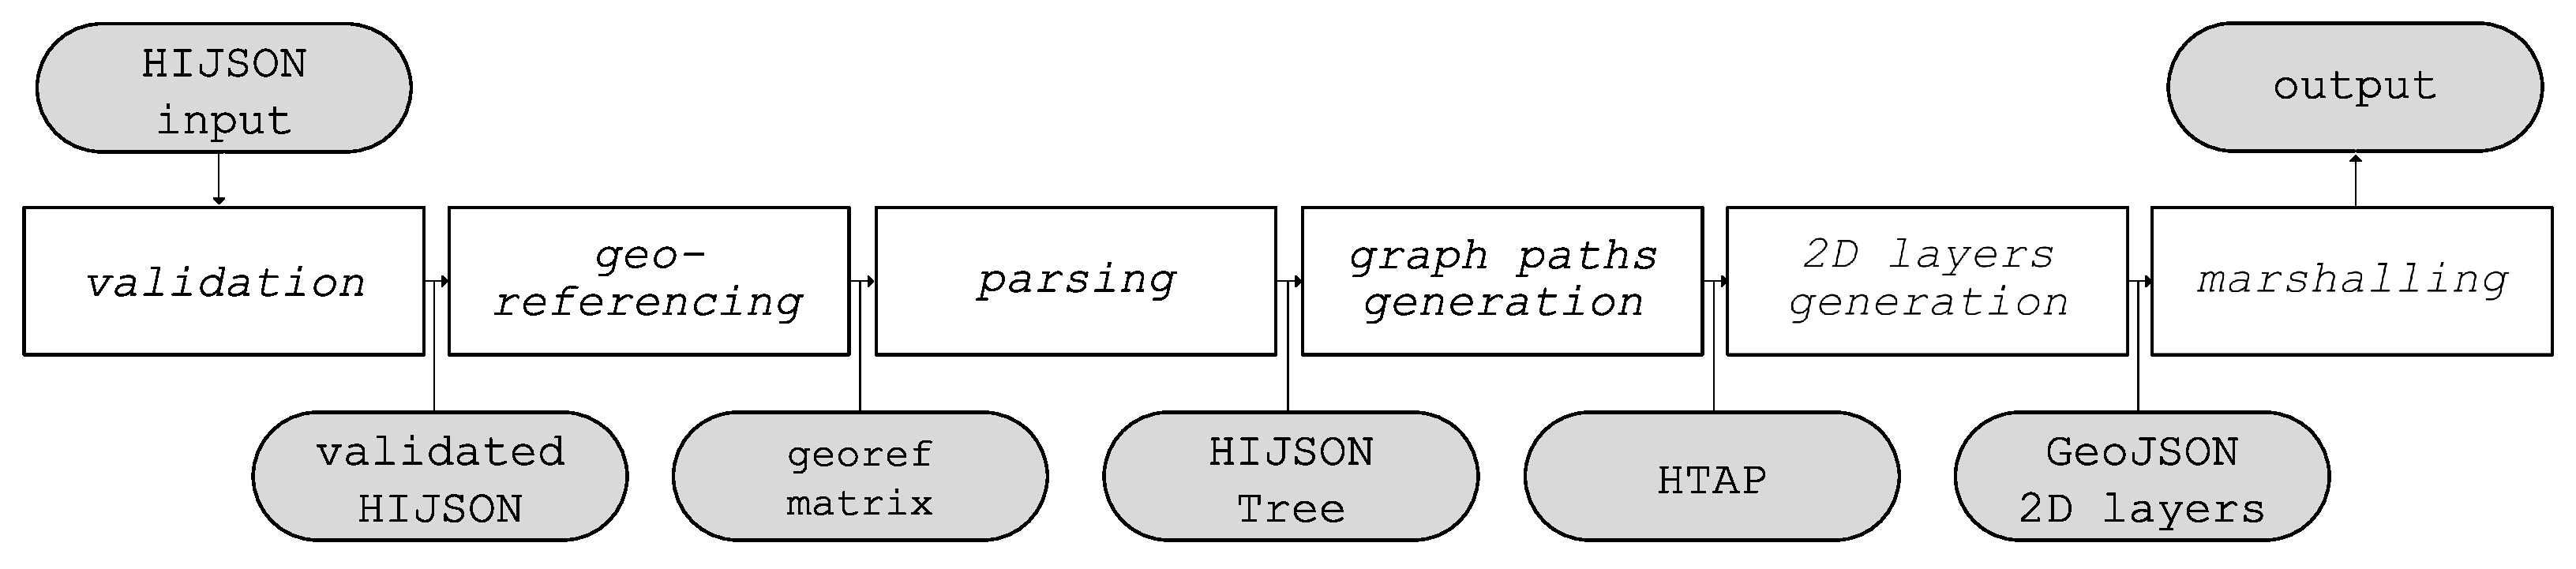
\includegraphics[width=\linewidth]{images/pipeline}
 \caption{HIJSON Toolkit processing pipeline.}
 \label{fig:pipeline}
\end{figure}


\subsubsection{Automatic generation of valid paths}

Figure~\ref{fig:graph-generation} describes the main steps of the algorithm.
The graph generated, although non optimal, ensures a complete coverage of the
surface while limiting the number of generated nodes. The resulting graph is
weighted on the edges with nodes distances. 
The graph of paths allows for calculations of directions between any two given
nodes. Although different approaches have been explored [3], a very classical
solution has been selected in this case, so directions are actually computed
client-side by applying the Dijkstra algorithm to the graph.
Taking advantage of the hierarchical structure of the HIJSON document, and
according to the divide et impera approach, the problem of paths generation is
split in several sub-problems, which consist in the computation of the sub-
graphs relative to each individual space, more generally a single room.

\begin{figure}[h]
 \centering
 \begin{subfigure}[b]{0.1\textwidth}
 \includegraphics[width=\textwidth]{images/graph-new-1}
 \end{subfigure}
 ~
 \begin{subfigure}[b]{0.1\textwidth}
 \includegraphics[width=\textwidth]{images/graph-new-2}
 \end{subfigure}
 ~
 \begin{subfigure}[b]{0.1\textwidth}
 \includegraphics[width=\textwidth]{images/graph-new-3}
 \end{subfigure}
 ~
 \begin{subfigure}[b]{0.1\textwidth}
 \includegraphics[width=\textwidth]{images/graph-new-4}
 \end{subfigure}
 
 \caption{graph of paths generation: 
 (a) detection of obstacles and computation of walkable area; 
 (b) triangulation of walkable area; 
 (c) identification of graph nodes; 
 (d) junction of nodes.
 }
 \label{fig:graph-generation}
\end{figure}

\subsubsection{HIJSON Class definition}

To make better use of the possibilities offered by the HIJSON Toolkit and by
the HIJSON document format, some custom dynamic behaviors can be described.
These behaviors encapsulate the specificities relative to communication
protocols with the sensors, as well as to features of user interaction. The
interface for such behavior is the HIJSON Class. Every Element of the input
HIJSON document has a dynamic counterpart, a running instance called  Node,
instantiated according to the corresponding Class via reflection methods, see figure~\ref{fig:el-class-node}.

\begin{figure}[h]
 \centering
 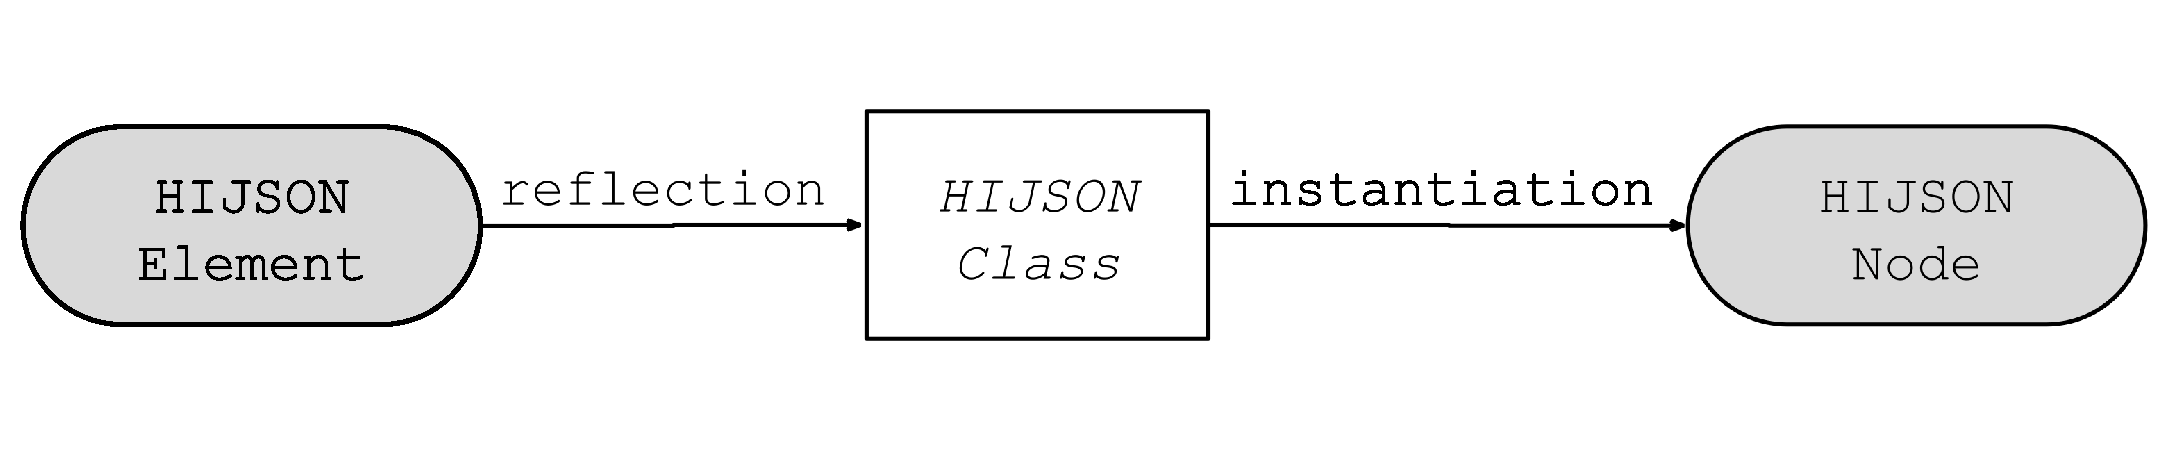
\includegraphics[width=0.6\linewidth]{images/element-class-node}
 \caption{HIJSON Element/Class/Node relashionships.}
 \label{fig:el-class-node}
\end{figure}

User's needs for new indoor elements, greatly different sensor equipments,
alternative representations of 2D or 3D viewports are accepted by the
definition of new HIJSON Classes, that so provide single-point custom
extensions of the Toolkit capabilities.

\subsection{FIVE web framework}

The  \emph{Framework for Interactive Visual Environments} (FIVE), responds to the needs of an extendable, customizable,
and scalable web framework which provides at the same time IoT monitoring,
realtime multi-person tracking and cross-storey user navigation.

Expandability and customizability derive from both design choices and HIJSON
inherent characteristics, i.e. the possibility of semantic extensions.
Scalability is directly borrowed from technologies used for software
development: JavaScript language, using Node.js, in particular Express.js as
backend framework, exploiting the power of WebSocket protocol through the
Socket.io library.

Being supported by the web-as-a-platform, the framework exposes also an high
availability: it is so simple to use as to visit a website, both from desktop
or mobile devices, without explicit requirements to install any software
package from proprietary stores|access to which is often denied from business
devices.

\subsubsection{Applications}

The Framework has been designed with focus on two different kind of users: the
Explorer and the Supervisor. They have different requirements and are likely
equipped with different devices: while the Supervisor monitors the indoor
environment through a desktop workstation, the Explorer has a smartphone
available and needs to be routed across the building. In both cases, the web
platform ensures a perfect alignment with the BYOD (Bring Your Own Device)
approach, nowadays often supported by companies that encourage employees to
use personal devices.


\begin{figure}[htb]
\centering
\includegraphics[width=\linewidth]{images/2D-3D}
\caption{FRAME Web Framework UI}
\label{fig:web-framework-ui}
\end{figure}

\subsubsection{IoT monitoring}

An IoT monitoring application consists of an interface showing to the user, in
a single, integrated and centralized way, the information collected from all
the smart objects modelled in the HIJSON document. IoT monitoring application
provides bidirectional communication, since the interface let the user receive
information coming from smart objects while allowing him to send commands to
them.

As the name itself may suggest, it is an activity specifically performed by a
Supervisor user, but it can be also suitable to be deployed for the Explorer
user, since she can take advantage of the interactive information coming from
the surroundings objects while she moves across the indoor environment.

Monitoring different smart objects may require different ways to visualize
and/or send data and commands. In particular, the user interface is
characterized by a dual-display mode, that allows the user to see at the same
time a 2D map that gives an overall glance in a simplified plan, and a 3D
virtual environment to navigate into, as shown in Figure 6.

Alongside with typical smart objects, suitable to deal with like thermostats,
where the user can read the room temperature and turn the heating on/off,
other kinds of objects, that are not properly considered ``smart", can be
integrated into the HIJSON environment. It is the case, for example, of fire
extinguishers, that are able to show the date of their last check, stored in a
database.

\subsubsection{Realtime multi-person tracking} Realtime multi-person tracking
allows a Supervisor to monitor the current real position of people inside the
building. This kind of task can be useful for several reasons, including
security, logistics or to supervise composite operative workflows. Each device
equipped with the Explorer application is in charge of locating itself,
interacting with the indoor positioning system, and notifying the current
position in continuos mode. Evidence of the people position is given to the
Supervisor both into a 2D map and an immersive 3D virtual environment (see
Figure 6).

\subsubsection{Cross-storey user navigation} The FRAME Framework also provides
the capability to give directions to Explorer users that must move across the
indoor environment. The user specifies a starting and an ending point and the
system provides him with a valid connection path. This feature strongly rely
on the graph of paths generated by the Toolkit, so starting and ending points
must be nodes of the graph. Connection nodes are introduced to represent
stairs or elevators, enabling cross-storey paths to be computed. Since paths
can span more than one storey, the most effective way to display them to the
user is to show the connection nodes visualized in one or more 2D maps.


%-------------------------------------------------------------------------
\section{Conclusions}

In this paper a novel document format, named HIJSON, for indoor cartographical
descriptions has been introduced. Utilization of local metric coordinate
system, avoiding the manipulation of global geographical coordinates, really
inconvenient when dealing with indoor spaces and objects, greatly enhances the
modeling and rendering of the document content. Currently, we produce the
HIJSON document from a python script using two libraries for geometric
computing (pyplasm and larcc). The modeling process can be further
improved by implementing a LAR-based graphical editor to assist the user
during the description of the indoor space. The realization of such an editor
is already in our plans. On the basis of this representation a virtual web
environment can be rebuilt working as a unifying platform to run a bunch of
different applications. The reference architecture of such a platform has been
also implemented and described in this work. The architecture supports a whole
range of applications: IoT monitoring, realtime multi-person tracking and user
crossstorey navigation are already implemented and described. A very
convenient way to extend the representation capabilities of smart objects is
also mentioned as semantic extensions. These extensions, which affects both
document format and its web framework, might be easily collected in a public
repository. Community could both use public available extensions or contribute
by mapping new (smart) objects inside the HIJSON document format.

%-------------------------------------------------------------------------

%\bibliographystyle{eg-alpha}
\bibliographystyle{eg-alpha-doi}

\bibliography{doceng2015}


\tableofcontents


\end{document}
